
\section{8/16(三)上午:流程控制-迴圈}

\subsection{迴圈}
\subsubsection {while}
\begin{enumerate}
	\item 講解︰JA-003:1+2+3+...+100
		\begin{enumerate}
			\item 題目說明:
			\subitem 使用 while 迴圈計算 1+2+3+...+100
			
			\item 解題思維:
			\begin{enumerate}
				\item 宣告一個初始值為零的變數sum=0,準備進行累加。
				\item 使用while迴圈,當符合while的執行條件(n<100)時,會重複執行累加計算,累加完之後會更新n的值,當n不滿足執行條件時,結束迴圈。
				
			\end{enumerate}
				\begin{cppcode}
				#include <iostream>
				
				using namespace std;
				
				int main()
				{
					int n=1, sum=0;
					while (n<=100) {
						sum += n; // 累加
						n++; // 更新n
					}
					cout << sum;
					return 0;
				}
				
			\end{cppcode}
		\end{enumerate}
		
	\item 練習:JA-004︰1+3+5+...+99
		\begin{enumerate}
			\item 題目說明:
			\subitem 使用 while 迴圈計算 1+3+5+...+99
			
			\item 解題思維:
			\subitem 使用while迴圈進行累加,只要(n<100)就對sum進行累加,每次累加完後,n加上2。
			
			\item 程式碼:
			\begin{cppcode}
				#include <iostream>
				
				using namespace std;
				
				int main()
				{
					int n=1, sum=0;
					while (n<100) {
						sum += n;
						n += 2;
					}
					cout << sum;
					return 0;
				}
				
			\end{cppcode}
		\end{enumerate}
	
\end{enumerate}

\subsubsection {for}
\begin{enumerate}
	\item 講解︰JA-005:1+2+3+...+100
		\begin{enumerate}
			\item 題目說明:
			\subitem 使用 for 迴圈計算 1+2+3+...+100
			
			\item 解題思維:
			\subitem for迴圈的用法是for(起始值; 條件式; 更新值),本題的for迴圈寫法如下:
			\begin{inside}
				for (int i=1; i<=100; i++) sum += i;
			\end{inside}
			意思是:i的起始值是1,當i<=100這個條件成立時的時候,會重複執行累加(sum += i;),並在累加完後更新i的值(i++)。此迴圈總共回會複執行100次累加的計算。
			
			\item 程式碼:
			\begin{cppcode}
				#include <iostream>
				
				using namespace std;
				
				int main()
				{
					int sum=0;
					for (int i=1; i<=100; i++) sum += i;
					cout << sum;
					return 0;
				}
				
			\end{cppcode}
		\end{enumerate}
	
	\item 練習︰JA-006:1+3+5+...+99
		\begin{enumerate}
			\item 題目說明:
			\subitem 使用 for 迴圈計算 1+3+5+...+99
			
			\item 解題思維:
			\subitem 使用for迴圈進行累加,只要(n<100)就對sum進行累加,n每次更新都加2。
			
			\item 程式碼:
			\begin{cppcode}
			#include <iostream>
			
			using namespace std;
			
			int main()
			{
				int sum=0;
				for (int i=1; i<100; i+=2) sum += i;
				cout << sum;
				return 0;
			}
				
			\end{cppcode}
		\end{enumerate}
	
\end{enumerate}

\subsubsection {應用題}
\begin{enumerate}
	\item 講解︰JT-04:印三角形函數
		\begin{enumerate}
			\item 題目說明:
			\subitem 輸入N,印出N列的星號(*),其中第I列有I個星,如執行範例所示。
			\subitem 範例輸入:5
			\subitem 範例輸出:
				\begin{figure}[H]
					\centering
					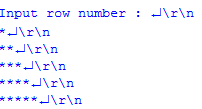
\includegraphics{fig/JT04fig}
				\end{figure}
			
			\item 解題思維:
			\subitem 
				這題需要使用雙重for迴圈。第一個迴圈計算現在要印第幾列,第二個迴圈計算要印幾個星。
			\item 程式碼:
			\begin{cppcode}
				#include <stdio.h>
				
				int main()
				{
					int n, i, j;
					printf("Input row number : \n");
					scanf("%d", &n);
					for (i=1; i<=n; i++) { // 迴圈1:第i列
						for(j=0; j<i; j++) { // 迴圈2:印i個星
							printf("*");
						}
						printf("\n");
					}
					return 0;
				}
					
			\end{cppcode}
		\end{enumerate}

	\item 練習︰JP-010-2:印倒三角形(無空白)
		\begin{enumerate}
			\item 題目說明:
			\subitem 輸入正整數n<=20,輸出一個n層的倒三角形。
			\subitem 範例輸入:5
			\subitem 範例輸出:
			\begin{figure}[H]
				\centering
				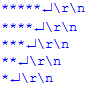
\includegraphics{fig/JP010fig}
			\end{figure}
			\item 解題思維:
			\subitem 印倒三角形時,第一列有n個星,下一列有n-1個星,以此列推,每換一列就少一個星,所以這題是要使用for迴圈來倒數。
			\item 程式碼:
			\begin{cppcode}
			#include <cstdio>
			
			int main()
			{
				int n, i, j;
				scanf("%d", &n);
				for (i=n; i>0; i--) { // 迴圈1:計算此列有i個星
					for(j=i; j>0; j--) { // 迴圈2:印出i個星
						printf("*");
					}
					printf("\n");
				}
				return 0;
			}
				
			\end{cppcode}
		\end{enumerate}
	
	\item 挑戰︰JT-40印等腰三角形
		\begin{enumerate}
			\item 題目說明:
			\subitem 輸入N,印出一個N列的等腰三角形,其中第I列有2*I-1個\#,如程式範例結果所示。
			\subitem 範例輸入:5
			\subitem 範例輸出:
			\begin{figure}[H]
				\centering
				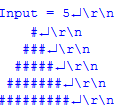
\includegraphics{fig/JT40fig}
			\end{figure}
			
			\item 解題思維:
			\begin{enumerate}
				\item 因為要印出N列,所以先寫一個執行N次的for迴圈,用變數row來計算現在是第幾列。
				\item 第row列要印出(n-row)個``空白",及(2*row-1)個``\#",所以分別用兩個for迴圈印``空白"及``\#"。
			\end{enumerate}
			
			\item 程式碼:
			\begin{cppcode}
				#include <stdio.h>
				
				int main()
				{
					int i, row, n;
					scanf("%d", &n);
					printf("Input = %d\n", n);
					for (row=1; row<=n; row++) {
						for (i=0; i<n-row; i++) printf(" ");
						for (i=0; i<2*row-1; i++) printf("#");
						printf("\n");
					}
					return 0;
				}
				
			\end{cppcode}
		\end{enumerate}

\end{enumerate}

\subsubsection {do while {\color{blue}(若有多餘時間)}}

\section{8/16(三)下午:函數}
\subsection{printf()格式輸出}
\begin{enumerate}
	\item 講解︰JB-02:九九乘法表
		\begin{enumerate}
			\item 題目說明:
			\subitem 印出如輸出之九九乘法表。
			\begin{figure}[h]
				\centering
				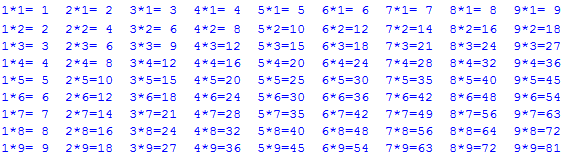
\includegraphics[width=12cm]{fig/JB02fig}
			\end{figure}
			\item 解題思維:
			\begin{enumerate}
				\item 先看第一列,會變動的數是``被乘數",而且變動是有規律的1,2,3...,9,所以我們寫一個會執行9次的for迴圈,讓變數j從1跑到9。變數j就是要輸出的``被乘數"。
				\begin{figure}[H]
					\centering
					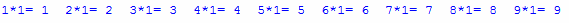
\includegraphics[width=12cm]{fig/JB02fig_2}
				\end{figure}
				\item 再來觀察``乘數",同一列的乘數是固定的,乘數隨著列改變,也就是說第i列的乘數是i。總共有9列,所以要寫一個會執行9次的for迴圈。變數i就是要輸出的``乘數"。
				\item ``乘積"只要將i, j 相乘就可以了。
				\item 這題使用printf()格式輸出比較容易。``\%2d"表示輸出時,會給這個整數兩給位數,當輸出的整數只有個位數的時候,十位數的位置會自動補上``空格"。
			\end{enumerate}
			
			\item 程式碼:
			\begin{cppcode}
			#include <cstdio>
			
			int main()
			{
				for (int i=1; i<=9; i++) {//第i列的乘數是i
					for(int j=1; j<=9; j++) {//每一列的被乘數j都從1~9
						printf("%d*%d=%2d  ", j, i, i*j);
					}
					printf("\n");
				}
				return 0;
			}
				
			\end{cppcode}
		\end{enumerate}
	
	\item 練習︰JA-007:九九乘法表 (兩排)
		\begin{enumerate}
			\item 題目說明:
			\subitem 印出九九乘法表,如輸出結果所示。
			\begin{figure}[h]
				\centering
				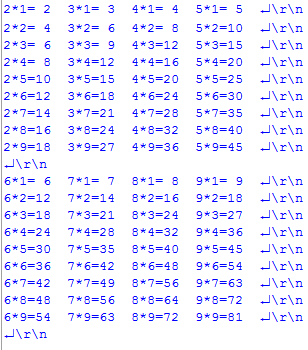
\includegraphics[height=6cm]{fig/JA007fig}
			\end{figure}
			\item 解題思維:
			\subitem 可以想成輸出兩個大群組的九九乘法表,當輸出第r (r=0, 1) 個群組時``被乘數"$=j+r\times4.$ (j=2, 3, 4, 5)。
			
			\item 程式碼:
			\begin{cppcode}
				#include <cstdio>
				
				int main()
				{
					for (int r=0; r<2; r++) {//兩個群組
						for (int i=1; i<=9; i++) {//第i列的乘數是i
							for(int j=2; j<=5; j++) {//被乘數=j+r*4
								printf("%d*%d=%2d  ", j+r*4, i, i*(j+r*4));
							}
							printf("\n");
						}
						printf("\n");
					}
					return 0;
				}
				
			\end{cppcode}
		\end{enumerate}
	
\end{enumerate}
\subsection{自訂函數}
\begin{enumerate}
	\item 講解︰JT-04印三角形函數
	\begin{enumerate}
		\item 題目說明:
		\subitem 輸入N,印出N列的星號(*),其中第I列有I個星,如執行範例所示。
		\subitem 範例輸入:5
		\subitem 範例輸出:
		\begin{figure}[H]
			\centering
			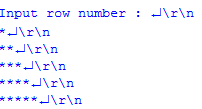
\includegraphics{fig/JT04fig}
		\end{figure}
		
		\item 解題思維:
		\begin{enumerate}
			\item 自己定義畫三角形的函數,使用這個函數時,需要輸入參數n,這樣函數才知道三角形有幾列。
			\item 將畫三角形的程式碼寫進函式裡,主程式main裡面只需要呼叫函數即可印出三角形。
		\end{enumerate}
		
		\item 程式碼:
		\begin{cppcode}
			#include <stdio.h>
			
			void triangle(int n);
			
			int main()
			{
				int n;
				printf("Input row number : \n");
				scanf("%d", &n);
				triangle(n);
				return 0;
			}
			
			void triangle(int n)
			{
				int i, j;
				for (i=1; i<=n; i++) {
					for (j=0; j<i; j++) { printf("*"); }
					printf("\n");
				}
			}
			
		\end{cppcode}
	\end{enumerate}
	
	\item 練習︰JP-010-2:印倒三角形(無空白)
	\begin{enumerate}
		\item 題目說明:
		\subitem 輸入正整數n<=20,輸出一個n層的倒三角形。
		\subitem 範例輸入:5
		\subitem 範例輸出:
		\begin{figure}[H]
			\centering
			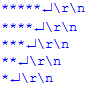
\includegraphics{fig/JP010fig}
		\end{figure}
		\item 解題思維:
		\begin{enumerate}
			\item 自己定義畫三角形的函數,使用這個函數時,需要輸入參數n,這樣函數才知道三角形有幾列。
			\item 將畫倒三角形的程式碼寫進函式裡,主程式main裡面只需要呼叫函數即可印出三角形。
		\end{enumerate}
		\item 程式碼:
		\begin{cppcode}
			#include <cstdio>
			
			void plot(int n);
			
			int main()
			{
				int n;
				scanf("%d", &n);
				plot(n);
				return 0;
			}
			
			void plot(int n)
			{
				int i, j;
				for (i=n; i>0; i--) {
					for(j=i; j>0; j--) {
						printf("*");
					}
					printf("\n");
				}
			}		
		\end{cppcode}
	\end{enumerate}
	
	\item 練習︰JT-40:印等腰三角形
		\begin{enumerate}
			\item 題目說明:
			\subitem 輸入N,印出一個N列的等腰三角形,其中第I列有2*I-1個\#,如程式範例結果所示。
			\subitem 範例輸入:5
			\subitem 範例輸出:
			\begin{figure}[H]
				\centering
				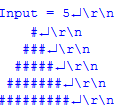
\includegraphics{fig/JT40fig}
			\end{figure}
			
			\item 解題思維:
			\begin{enumerate}
				\item 自己定義畫三角形的函數,使用這個函數時,需要輸入參數n,這樣函數才知道三角形有幾列。
				\item 將畫等腰三角形的程式碼寫進函式裡,主程式main裡面只需要呼叫函數即可印出三角形。
			\end{enumerate}
			
			\item 程式碼:
			\begin{cppcode}
				#include <stdio.h>
				
				void plot(int n);
				
				int main()
				{
					int n;
					scanf("%d", &n);
					printf("Input = %d\n", n);
					plot(n);
					
					return 0;
				}
				
				void plot(int n)
				{
					int i, row;
					for (row=1; row<=n; row++) {
						for (i=0; i<n-row; i++) printf(" ");
						for (i=0; i<2*row-1; i++) printf("#");
						printf("\n");
					}
				}
				
				
			\end{cppcode}
		\end{enumerate}
		
	
	
	\item 挑戰︰JT61:Game Over
		\begin{enumerate}
			\item 題目說明:
			\subitem 輸入整數 m 和 n,輸出以 \# 排成框,中間為 Game Over 之圖案,其中 m 為 G 之
			前和 r 之後與邊界的空格數,n 為文字與上下邊界的空格數。例如輸入 2 1,則輸出為
			\begin{figure}[h]
			\centering
			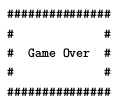
\includegraphics{fig/game_over_fig}
			\end{figure}
			\item 解題思維:
			\begin{enumerate}
				\item 第1列有11+2m個\#。
				\item 接下來n列頭尾是\#,中間有9+2m個空白。
				\item 再下一列是\#加m個空白,加Game Over,加m個空白和\#。
				\item 接下來n列頭尾是\#,中間有9+2m個空白。
				\item 最後一列有11+2m個\#。
			\end{enumerate}
			\item 程式碼:
		\begin{cppcode}
			#include <iostream>
			
			using namespace std;
			
			int main()
			{
				int m, n;
				cin >> m >> n;
				for (int i=0; i<11+2*m; i++) cout << "#"; // Row 1
				cout << endl;
				for (int r=0; r<n; r++) { // Next n rows
					cout << "#";
					for (int i=0; i<9+2*m; i++) cout << " ";
					cout << "#" << endl;
				}
				cout << "#"; // Middle row
				for (int i=0; i<m; i++) cout << " ";
				cout << "Game Over";
				for (int i=0; i<m; i++) cout << " ";
				cout << "#" << endl;
				for (int r=0; r<n; r++) { // Next n rows
					cout << "#";
					for (int i=0; i<9+2*m; i++) cout << " ";
					cout << "#" << endl;
				}
				for (int i=0; i<11+2*m; i++) cout << "#"; // Last row
				cout << endl;
				return 0;
			}
		
	\end{cppcode}
				
		\end{enumerate}
	
\end{enumerate}

